\documentclass[conference]{IEEEtran}\usepackage[T1]{fontenc}\usepackage[utf8]{inputenc}\usepackage{graphicx,booktabs}\begin{document}\title{Evaluating AI-Adaptive Learning in Higher Education Using a Simulated Randomized Trial}\author{\IEEEauthorblockN{Nurali Seifulla and Nurbakyt Sagidulla}\IEEEauthorblockA{Narxoz University, Almaty, Kazakhstan}}\maketitle\begin{abstract}Adaptive learning platforms can change both the sequence of exercises and the time students spend on them. Evaluating such a platform requires an analysis that distinguishes learning outcomes from operational performance. We specify a two-arm randomized study and evaluate its analysis pipeline using a seeded simulation of 140 university learners over eight weekly sessions. The primary outcome is the difference between arms in mean change from pre-test to post-test. Secondary measures include time on task, session quiz scores, response latency, and errors. Of 140 simulated learners, 133 completed both tests. The adaptive arm gained 2.95 more points on average than the traditional arm (95\% bootstrap interval 0.54 to 5.41) and spent 8.34 fewer minutes per evaluation session. Both contrasts reflect assumptions encoded in the generator. The analysis also detected elevated latency in both onboarding weeks and uncertainty around the operational error threshold. The resulting workflow connects event-level records to interpretable estimates and identifies the evidence required for a subsequent student trial.\end{abstract}\begin{IEEEkeywords}Adaptive learning, educational technology, randomized trials, simulation, learning analytics\end{IEEEkeywords}
\section{Introduction}\label{sec:intro}
Adaptive systems choose learning activities using information about a learner's progress. Studies of educational outcomes~\cite{ref1} and academic inequality~\cite{ref2} motivate measuring who completes an intervention as well as how much completers learn. Conceptual accounts~\cite{ref3} and work on university language instruction~\cite{ref4} illustrate how different implementations can share the label ``adaptive learning.'' Reviews of platform designs~\cite{ref5} and work on educational transformation~\cite{ref6} provide context for specifying a comparison at the level of one course module.


Pedagogical agents~\cite{ref7}, personalized AI agents~\cite{ref8}, adaptive learning experiences~\cite{ref9}, and higher-education assistants~\cite{ref10} represent different interventions. A review of adaptive e-learning~\cite{ref11} and a meta-analysis of intelligent tutoring systems~\cite{ref12} inform the broader question of effectiveness. For the proposed course study, the open measurement question is whether a difference in test-score gain can be estimated alongside time on task while retaining failed sessions and accounting for missing post-tests.


Our contributions are threefold.\begin{itemize}
\item We specify a stratified two-arm protocol with a common assessment and an explicit gain estimand.
\item We implement a reproducible analysis that links individual outcomes to session-level operational measures.
\item We exercise the workflow on a synthetic cohort and identify where design assumptions restrict interpretation.
\end{itemize}
Section~\ref{sec:methods} defines the protocol, Section~\ref{sec:results} reports the simulation, and Section~\ref{sec:limits} discusses validity and the next empirical test.



\section{Methodology}\label{sec:methods}
A. Design and estimand. The planned trial assigns individual students to a fixed-order course module or an AI-adaptive version using the same item bank, learning objectives, schedule, and assessment criteria. Allocation targets equal groups within terciles of baseline score. Week 0 supplies the pre-test, weeks 1--8 the learning sessions, and week 9 the post-test. Table~\ref{tab:settings} summarizes the analysis settings.

\begin{table}[!ht]\centering\caption{Simulation and analysis settings.}\label{tab:settings}\begin{tabular}{ll}\toprule Parameter & Specification \\ \midrule
Participants & 140 planned \\
Schedule & 8 sessions, weeks 1--2 warm-up \\
Bootstrap & 10,000 samples, seed 42 \\
Error / latency limits & 2\% / 1,000 ms (p95) \\
Attrition limit & 15\% per arm \\ \bottomrule\end{tabular}\end{table}
Eq.~\ref{eq:gain} defines individual gain and its between-arm contrast. Each score ranges from 0 to 100. The estimate uses students with both test scores. Positive values indicate larger gains in the adaptive arm. Time on task is averaged across each completer's successful evaluation sessions before comparing arms, so a learner with additional successful sessions does not receive extra weight.

\begin{equation}\Delta_i=X_i^{post}-X_i^{pre},\quad\hat{\tau}=\bar{\Delta}_{A}-\bar{\Delta}_{T}.\label{eq:gain}\end{equation}
B. Data generation and processing. Figure~\ref{fig:arch} traces the implemented system. With seed 42, the generator samples baseline ability, assigns groups, and draws gains conditional on group and baseline. It sets nominal mean gains to 12.0 and 15.5 points and evaluation-time medians to 62 and 54 minutes. The synthetic post-test is generated from baseline and gain. Session performance does not feed back into that post-test. A more favorable simulated gain therefore cannot validate the adaptive policy.

\begin{figure}[!ht]\centering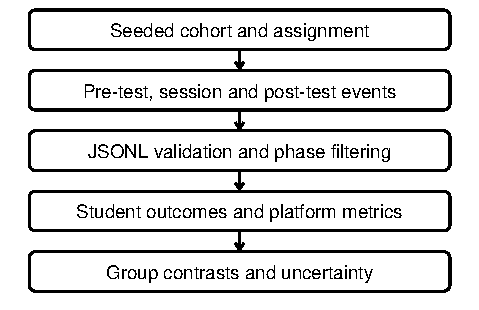
\includegraphics[width=.91\columnwidth]{architecture.pdf}\caption{Implemented simulation and analysis workflow.}\label{fig:arch}\end{figure}
The pipeline reads one event per JSON line. It checks score bounds, positive recorded times and latencies, and consistency between phase and session index. Failed sessions remain in the error-rate denominator. Successful sessions supply latency and quiz outcomes. Warm-up filtering applies to session summaries, while pre/post gain spans the entire study.


C. Inference. A two-sided Welch test assesses equality of mean gains. The decision rule requires both p $<$ 0.05 and a percentile bootstrap interval excluding zero. Each bootstrap draw samples learners with replacement within arms. Hedges' g standardizes the difference using the pooled standard deviation and a small-sample correction. ANCOVA adjusts post-test score for baseline and arm. A Mann--Whitney test checks sensitivity to the outcome distribution.



\section{Results and Discussion}\label{sec:results}
Figure~\ref{fig:weekly} tracks weekly quiz performance through onboarding and evaluation.
\begin{figure*}[!t]\centering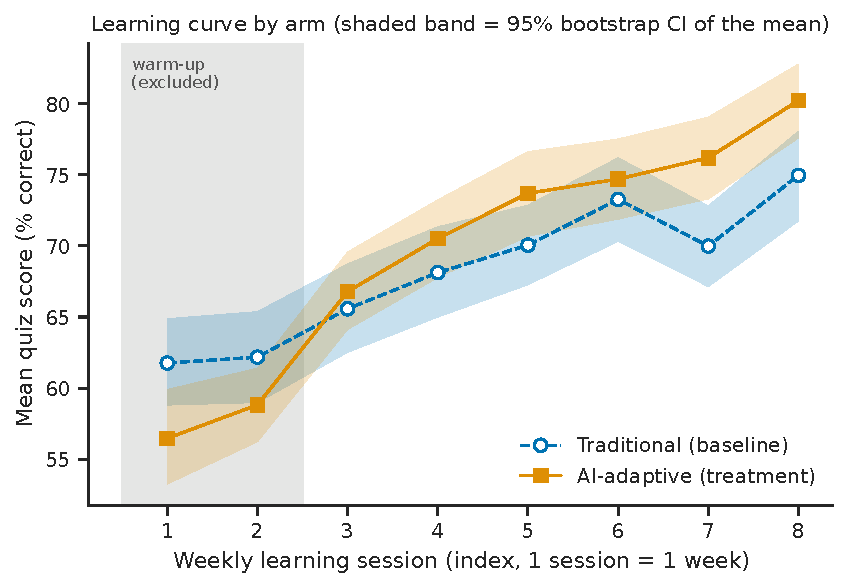
\includegraphics[width=.74\textwidth]{fig1_score_vs_session.pdf}\caption{Weekly quiz performance in the simulated cohort. Bands are pointwise 95\% bootstrap intervals. The shaded onboarding period is retained here to show the transition into the evaluation window.}\label{fig:weekly}\end{figure*}
A. Cohort and primary outcome. The log contains 140 pre-tests, 1,101 sessions, and 133 post-tests. The realized allocation was 71 traditional and 69 adaptive learners. Five traditional and two adaptive learners lacked a post-test. Figure~\ref{fig:gain} shows the individual gains behind the group means in Table~\ref{tab:results}. The distributions overlap despite a positive mean contrast.

\begin{table}[!ht]\centering\caption{Outcomes for the simulated cohort.}\label{tab:results}\begin{tabular}{lll}\toprule Metric & Traditional & Adaptive \\ \midrule
Completed / assigned & 66 / 71 & 67 / 69 \\
Gain, mean $\pm$ SD & 12.24 $\pm$ 7.30 & 15.19 $\pm$ 7.10 \\
Time, min/session & 62.73 & 54.39 \\
Quiz median, \% & 70.0 & 74.0 \\
Latency p95, ms & 399 & 621 \\
Errors / sessions & 3 / 412 & 5 / 409 \\
Attrition, \% & 7.04 & 2.90 \\ \bottomrule\end{tabular}\end{table}\begin{figure}[!ht]\centering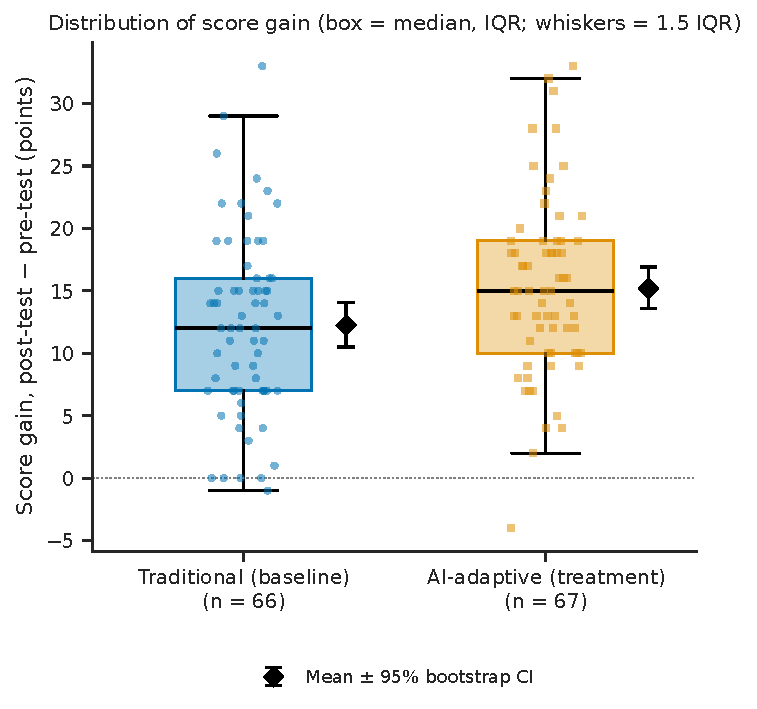
\includegraphics[width=.91\columnwidth]{fig2_distribution_boxplot.pdf}\caption{Individual simulated score gains by arm.}\label{fig:gain}\end{figure}
The mean contrast was 2.95 points (95\% bootstrap CI 0.54--5.41). Welch's t was 2.36 with 130.75 degrees of freedom (p = 0.0196), and Hedges' g was 0.41. The baseline-adjusted estimate was 2.93 points (95\% CI 0.47--5.40). The Mann--Whitney comparison gave p = 0.0176. These results satisfy the decision rule within this simulation. Agreement across analyses reflects the same generated cohort and provides a check on implementation.


B. Learning time and platform operation. After 280 onboarding sessions were set aside, 821 evaluation sessions remained. Eight recorded errors, leaving 813 successful sessions for session-level performance summaries. Completers in the adaptive arm spent 8.34 fewer minutes per session on average. This measure captures task duration. The study did not define a mastery threshold or observe time until mastery.


Figure~\ref{fig:lat} shows why phase matters. Adaptive p95 latency reached 2,060 ms in week 1 and 1,260 ms in week 2, both above the 1,000 ms reference. Across evaluation weeks, p95 fell to 621 ms in the adaptive arm and 399 ms in the traditional arm. Error proportions were below 2\% in both arms, but Wilson upper limits reached 2.83\% and 2.12\%, respectively. Point estimates alone cannot establish that the underlying rates meet the target.

\begin{figure}[!ht]\centering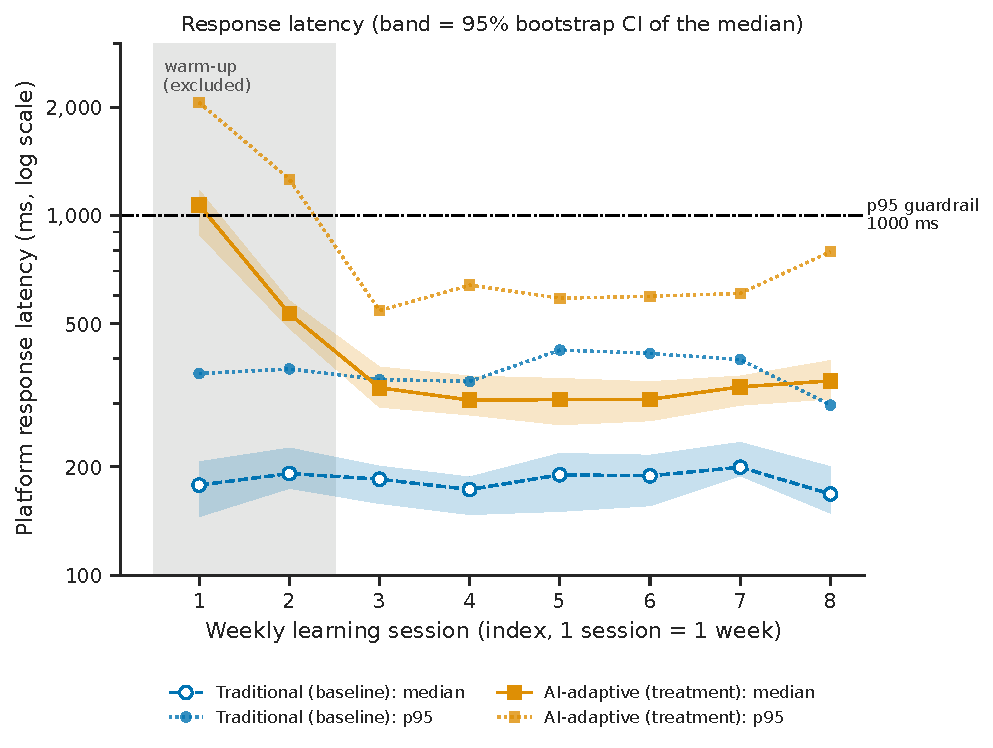
\includegraphics[width=.91\columnwidth]{fig3_latency_vs_session.pdf}\caption{Latency by week, including onboarding.}\label{fig:lat}\end{figure}

\subsection{Weekly learning trajectory}
Figure~\ref{fig:weekly} shows weekly quiz means computed from successful sessions. The trajectory supplies a different view of the study than the pre/post comparison. A single learner contributes one score per successful week, and the number observed can change as errors and dropout occur. Each band summarizes uncertainty about the mean for that arm and week. Comparisons across weeks therefore depend on the composition of the observed group as well as on changes within learners.



The adaptive group starts at 56.5\% in week 1 and reaches 80.2\% in week 8. The corresponding traditional means are 61.8\% and 75.0\%. At week 3 the difference is only 1.2 percentage points, compared with 5.3 points in week 8. The generator imposes a cold-start penalty during onboarding and a steeper subsequent trajectory for the adaptive arm. A reversal in the plotted ordering is consequently an expected feature of the simulation. A formal test of a treatment-by-week interaction would require a model for repeated measurements and a prespecified contrast.

\subsection{Operational interpretation}
The denominators matter for both learning and reliability. Traditional learners generated 412 evaluation sessions, of which 409 were successful. Adaptive learners generated 409, of which 404 were successful. A failed request contributes an error observation but supplies no time or quiz score. Including such a request as a zero-minute session would make the group with more failures appear faster. Excluding it from the error denominator would distort the reliability estimate in the opposite direction. The pipeline retains both denominators so that a reviewer can reconstruct each comparison.

The interpretation of time also depends on the unit of analysis. An average of all recorded session times gives greater weight to learners who contribute more successful sessions. Averaging first within learner gives each completer the same weight in the group mean. This choice aligns the time comparison with the unit of assignment. It leaves open whether a student who withdrew would have completed subsequent tasks more slowly or more quickly. A future deployment should record withdrawal reasons and preserve failed attempts alongside the successful-session measurements.

\section{Limitations and Conclusion}\label{sec:limits}
Internal validity. The simulator specifies group effects on outcomes, time, latency, and errors. A single seed tests one realization. Complete-case analysis omits seven learners and can introduce selection bias when dropout depends on achievement. Repeated session observations from the same learner may be correlated. Intervals obtained by pooling individual sessions can understate uncertainty for session-level summaries.


External validity. The protocol models one course over eight weeks. Neither longer-term retention nor transfer to other courses was observed. The learner model in the domain specification describes a candidate adaptive mechanism. This simulation did not train it or measure prediction accuracy. The deferred question about which algorithm settings predict learning difficulties requires item-level predictions, responses, and independent validation.


For the primary research question, the simulated comparison yielded a larger gain and shorter session time in the adaptive arm. Its empirical counterpart remains open. A prospective study would require ethics approval and consent, prespecified assignment and analysis, equivalent assessments, and a real platform export. The next analysis should assess sensitivity to missing post-tests and use learner-level resampling for longitudinal session summaries.


\bibliographystyle{IEEEtran}\bibliography{references}\end{document}